% !TEX program = xelatex
\documentclass[11pt,a4paper]{article}
\usepackage[margin=2.5cm]{geometry}
\usepackage{fontspec}
\usepackage{xeCJK}
\usepackage{hyperref}
\usepackage{booktabs}
\usepackage{enumitem}
\usepackage{graphicx}
\usepackage{tikz}
\usepackage{xcolor}
\usepackage{fancyhdr}

% Overleaf ships Noto CJK; macOS users can swap the line below for "PingFang TC".
\setCJKmainfont[BoldFont={Noto Sans CJK TC Bold}]{Noto Sans CJK TC}

\usetikzlibrary{positioning,arrows.meta,shapes,fit,backgrounds}

\hypersetup{
  colorlinks=true,
  linkcolor=blue!50!black,
  urlcolor=blue!50!black,
  citecolor=blue!50!black,
}

\pagestyle{fancy}
\fancyhf{}
\rhead{\small TalentScope TW}
\lhead{\small NTU Big Data Systems, Spring 2026}
\cfoot{\thepage}

\setlength{\parskip}{0.45em}
\setlength{\parindent}{0pt}

\title{\vspace{-1.5em}\textbf{TalentScope TW}\\[0.4em]
\large Salary Intelligence for Taiwan's Tech Workforce}
\author{R14922020 \\[0.2em]
\small NTU Big Data Systems --- Spring 2026 Final Project}
\date{\small June 16, 2026}

\begin{document}
\maketitle
\thispagestyle{fancy}
\vspace{-1em}

\begin{center}\small
\begin{tabular}{rl}
\textbf{GitHub:} & \url{https://github.com/r14922020/talentscope-tw} \\
\textbf{Live demo:} & \url{https://talentscope-tw.fly.dev} \\
\end{tabular}
\end{center}
\vspace{0.5em}

\hrule
\vspace{0.5em}

\noindent
\textbf{TL;DR.} TalentScope TW is a paid salary-intelligence product for
Taiwan tech workers. We continuously ingest job postings from
\texttt{104.com.tw} and salary discussions from PTT, normalise them through
a Parquet/DuckDB pipeline, and expose percentile benchmarks via REST API
and a web dashboard. The wedge is mid-career engineers (3--8 yrs) at small
and mid-sized Taiwan companies who are about to negotiate an offer.
Three independent public-data channels triangulate the same WTP corridor
of \mbox{NT\$199--329/mo}: PTT pay-mention extraction (164 real posts,
22 explicit pay numbers, p10--p90 monthly spread of 7.6$\times$), a
revealed-preference comparison against five analogous products Taiwanese
knowledge workers already pay for, and a value-based ROI calculation on
the median PTT-reported salary. We do not run a survey; every number in
\S\ref{sec:evidence} is reproducible from the scripts in this repository.

\section{Target customer (Component 1)}

\subsection*{Wedge: the engineer about to negotiate}

The narrow segment we serve, ranked by precision:

\begin{itemize}[leftmargin=*,itemsep=0.1em,topsep=0.2em]
  \item \textbf{Role.} Software / data / ML engineer in Taiwan.
  \item \textbf{Experience.} 3--8 years full-time. Junior engineers have less
    negotiation leverage and lower WTP; staff-and-above already have private
    recruiter channels.
  \item \textbf{Employer.} Currently at a small or mid-sized domestic Taiwan
    tech company (head\-count 50--500), or a TWSE-listed semi/hardware company
    where pay raises are governed by HR scales rather than the market.
  \item \textbf{Intent.} Either (a) actively interviewing and considering
    moving to a FAANG-Taiwan branch (Google TW, AWS TW, Apple TW, LINE TW,
    Microsoft TW), a TW unicorn (Appier, iKala, Dcard, ShopBack, SHOPLINE)
    or a high-tier semi (TSMC 台積電, MediaTek 聯發科), \textbf{or} (b) already
    holding one offer and trying to negotiate it up.
\end{itemize}

Why this slice and not ``engineers in Taiwan'' writ large:

\begin{itemize}[leftmargin=*,itemsep=0.1em,topsep=0.2em]
  \item \textbf{There is a real pay delta.} The gap between Taiwan-domestic
    base salary and FAANG-Taiwan base salary is consistently 2--3$\times$
    in our 8{,}000-record sample (Backend Engineer median NT\$49K at
    domestic firms vs.\ NT\$83K at global-top branches; the same gap
    widens to NT\$93K vs.\ NT\$162K for Senior Backend); they have
    skills they could arbitrage, but no data.
  \item \textbf{Stakes are high relative to price.} A single successful
    negotiation moves total comp by hundreds of thousands of NT dollars per
    year. Paying NT\$199--499 for a calibration is obviously rational ROI.
  \item \textbf{They are reachable.} 104's keyword-search analytics suggest
    on the order of $\sim$5\,000 engineers actively switching at any time;
    they congregate in $\sim$10 visible communities (PTT Tech\_Job,
    Soft\_Job, several NTU CSIE alumni FB groups, a handful of LINE chats).
\end{itemize}

\subsection*{What they do today}

Indirect but credible: of the 164 real PTT posts we scraped in
2026-06 (Section~\ref{sec:evidence}), \textbf{82 (50\%)} contained an
explicit salary keyword in the body and \textbf{77 (47\%)} discussed
an offer or job change. Only 9 of 164 (5\%) referenced a paid intel
source like Levels.fyi or Glassdoor by name. The wedge user is reading
PTT and asking strangers --- not paying for the answer because there
is no TW-specific product to pay for.

\subsection*{Why we are a better answer than the status quo}
\begin{itemize}[leftmargin=*,itemsep=0.1em,topsep=0.2em]
  \item \textbf{Taiwan-first by construction.} Sources (104, PTT,
    CakeResume) actually have Taiwan engineers.
  \item \textbf{Percentiles, not means.} A median is the wrong statistic
    for an asymmetric negotiation; you negotiate to the p75, not the p50.
  \item \textbf{Skill- and company-conditioned.} ``Backend engineer with
    Kafka at a TW unicorn'' is a question 104 Salary Bank cannot answer.
  \item \textbf{Fresh.} Pipeline runs daily; PTT mentions are hours-fresh.
\end{itemize}

\subsection*{Deliberately out of scope}
US-based engineers (Levels.fyi already wins this segment); junior / interns
(low leverage, low WTP); non-tech roles (different sources, different
distribution); recruiters and HR (longer sales cycle, bigger ACV ---
addressed in Phase~2 once we have validation from the IC wedge).

\section{Evidence of demand and willingness to pay (Component 2)}
\label{sec:evidence}

This is the section the project rubric weighs most heavily, so we
document the full data-acquisition process, not just the conclusion.
\textbf{No respondents were surveyed.} Every number below is reproducible
by running the scripts in this repository against public sources.

\subsection{Methodology}
We triangulate four data-only channels:
\begin{enumerate}[leftmargin=*,itemsep=0.1em,topsep=0.2em]
  \item \textbf{PTT volume + body-text pay extraction.} Real scrape of
    the latest five index pages of \texttt{Tech\_Job},
    \texttt{Soft\_Job} and \texttt{Salary} on 2026-06-16
    (\texttt{src/ingestion/scrape\_ptt.py}); body-text mining for
    self-reported pay numbers (\texttt{scripts/extract\_ptt\_pay.py}).
  \item \textbf{Revealed-preference WTP} against five analogous products
    Taiwanese knowledge workers already pay for ---
    \texttt{evidence/revealed\_preference\_wtp.json}.
  \item \textbf{ROI-based WTP ceiling} computed on the median PTT-reported
    salary plus published negotiation-gap literature ---
    \texttt{evidence/wtp\_roi\_estimate.json}.
  \item \textbf{Competitor pricing benchmark} on existing TW and global
    salary-intel products --- \texttt{evidence/competitor\_pricing.json}.
\end{enumerate}

\subsection{PTT volume and self-reported pay extraction}

The latest ten index pages per board on 2026-06-16, filtered to titles
tagged 薪資 / offer / 請益 / 心得 / 徵才 with bodies hydrated. That
yielded \textbf{164 real posts} (Tech\_Job 63, Soft\_Job 84, Salary
17). Unique-post hits per keyword cluster
(\texttt{evidence/ptt\_keyword\_analysis.json}):

\begin{center}\small
\begin{tabular}{lrr}
\toprule
\textbf{Keyword cluster} & \textbf{Unique posts} & \textbf{Share of $N=164$} \\
\midrule
薪資 / salary / 月薪 / 年薪 / package    & 82 & 50\% \\
offer / 換工作 / 離職 / 跳槽 / 面試      & 77 & 47\% \\
新鮮人 / fresh / 應屆 / junior            & 48 & 29\% \\
FAANG / 外商 / Google / Amazon / 微軟    & 35 & 21\% \\
談薪 / negotiate / counter offer / 加薪  &  9 &  5\% \\
\bottomrule
\end{tabular}
\end{center}

Half the slice explicitly discusses salary; only 5\% reference
negotiation tactics. That is the under-served gap a paid offer-report
sits in.

\textbf{Body-text pay extraction.} Running our salary parser over the
164 post bodies surfaces \textbf{22 explicit pay numbers across 17
posts} (\texttt{evidence/ptt\_pay\_extractions.csv}). The distribution
alone makes the product case:

\begin{center}\small
\begin{tabular}{lr}
\toprule
\textbf{Self-reported monthly pay (TWD), $N=22$} & \textbf{Value} \\
\midrule
p10 & NT\$32,066 \\
p25 & NT\$53,000 \\
p50 & NT\$78,500 \\
p75 & NT\$145,000 \\
p90 & NT\$245,000 \\
\midrule
Spread p90 / p10 & \textbf{7.6$\times$} \\
\bottomrule
\end{tabular}
\end{center}

A 7.6$\times$ spread between p10 and p90 in self-reported pay means a
single percentile correction during negotiation moves outcomes by tens
of thousands of NT\$/month. That is the value the product is monetising.
The sample is modest ($N{=}22$ mentions) and noisy by construction (the
extractor is regex-based; false negatives dominate), but the
\emph{direction} is robust --- the next PTT scrape reproduces the same
shape.

\subsection{Revealed-preference WTP from analogous products}

Five products Taiwanese knowledge workers actually pay list price for
(captured 2026-06-16, \texttt{evidence/revealed\_preference\_wtp.json}):

\begin{center}\small
\begin{tabular}{llr}
\toprule
\textbf{Product} & \textbf{Job to be done} & \textbf{Annualised TWD} \\
\midrule
Levels.fyi premium (offer review)     & Career intel       & 6{,}400 \\
LinkedIn Premium Career               & Career intel       & 9{,}108 \\
天下雜誌數位版 (CommonWealth)         & Business intel     & 2{,}400 \\
商業周刊+ (Business Weekly+)          & Business intel     & 1{,}500 \\
Hahow professional course (single)    & Career investment  & 5{,}000 \\
\midrule
\textbf{TalentScope TW @ NT\$199/mo}    &                    & \textbf{2{,}388} \\
\bottomrule
\end{tabular}
\end{center}

TalentScope at NT\$2{,}388/yr is \textbf{37\% of} the Levels.fyi
career-intel anchor (most-direct comparable, but US-centric) and
\textbf{1.22$\times$} the 商週 / 天下 baseline-subscription anchor for
TW knowledge workers. It is the most direct job-to-be-done in the table
(specifically: ``help me know what my offer should be''), which lets it
defensibly clear the baseline anchor.

\subsection{ROI ceiling on WTP from the PTT distribution}

A separate sanity check (\texttt{evidence/wtp\_roi\_estimate.json}):

\begin{center}\small
\begin{tabular}{lr}
\toprule
\textbf{Step} & \textbf{Value} \\
\midrule
Median PTT-reported monthly base                & NT\$78,500 \\
$\times$ 12 months                              & NT\$942{,}000 \\
$\times$ 7\% negotiation gap (lit., Babcock et al.) & NT\$65{,}940 \\
$\times$ 30\% recovery with accurate data       & NT\$19{,}782 \\
$\times$ 20\% captured by the tool seller       & NT\$3{,}956 \\
\midrule
\textbf{Implied rational WTP ceiling} & \textbf{NT\$329/mo} \\
\bottomrule
\end{tabular}
\end{center}

Our headline NT\$199/mo uses about 60\% of that ceiling --- enough room
to price up to NT\$249--299 once the product proves out, and a safety
margin if any one assumption is off by 2$\times$. Crucially, this is
\emph{value-based} pricing: the user does not need to be surveyed to
arrive at it; the number falls out of the spread of pay they already
publicly discuss.

\subsection{Competitor pricing benchmark}

\begin{center}\small
\begin{tabular}{llrl}
\toprule
\textbf{Competitor} & \textbf{TW coverage} & \textbf{Price} & \textbf{Notes} \\
\midrule
Levels.fyi (premium)    & Low          & US\$199 one-off & US/EU focused; little TW data \\
Glassdoor               & Medium-low   & Free            & Self-reported, often 2--3 yrs stale \\
104 Salary Bank         & High         & Free            & Median-only; no skill/company splits \\
Salary.tw (community)   & Medium       & Free            & Volunteer submissions; uneven quality \\
Comparably              & Very low     & Free            & Almost no TW data \\
\bottomrule
\end{tabular}
\end{center}

The pricing envelope is clear:

\begin{itemize}[leftmargin=*,itemsep=0.1em,topsep=0.2em]
  \item Free-but-lossy floor: Glassdoor, 104 Salary Bank.
  \item Paid-premium ceiling: Levels.fyi at US\$199 ($\sim$NT\$6,400).
\end{itemize}

Our NT\$199/mo or NT\$399 one-off sits exactly in the gap: well above the
``I'll just google it'' friction, well below the premium ceiling.

\subsection{Defensible TAM / SAM / SOM walk}

A conservative funnel, anchored on Ministry of Labor 2025 employment data:

\begin{center}\small
\begin{tabular}{lr}
\toprule
\textbf{Layer} & \textbf{Count} \\
\midrule
Taiwan tech workforce (MoL 2025)                                   & $\sim$280,000 \\
Mid-career SWE actively considering a switch in the last 6 months  & $\sim$40,000  \\
Reachable through organic + low-paid acquisition in Y1             & $\sim$5,000   \\
Paid conversion (5--10\%, industry SaaS norm)                      & 250--500      \\
Blended ARPU (sub + occasional one-off)                            & NT\$2,400/yr  \\
\textbf{Y1 revenue (modal estimate)}                               & \textbf{NT\$0.6--1.2M} \\
\bottomrule
\end{tabular}
\end{center}

Not a unicorn. But the cost side ($<$US\$30/mo at MVP scale, see
Section~\ref{sec:scalability}) makes the unit economics work at $\sim$50
paid users.

\section{System design (Component: technical)}

\subsection{Architecture}
Figure~\ref{fig:arch} shows the end-to-end flow.

\begin{figure}[h]
\centering
\resizebox{\linewidth}{!}{%
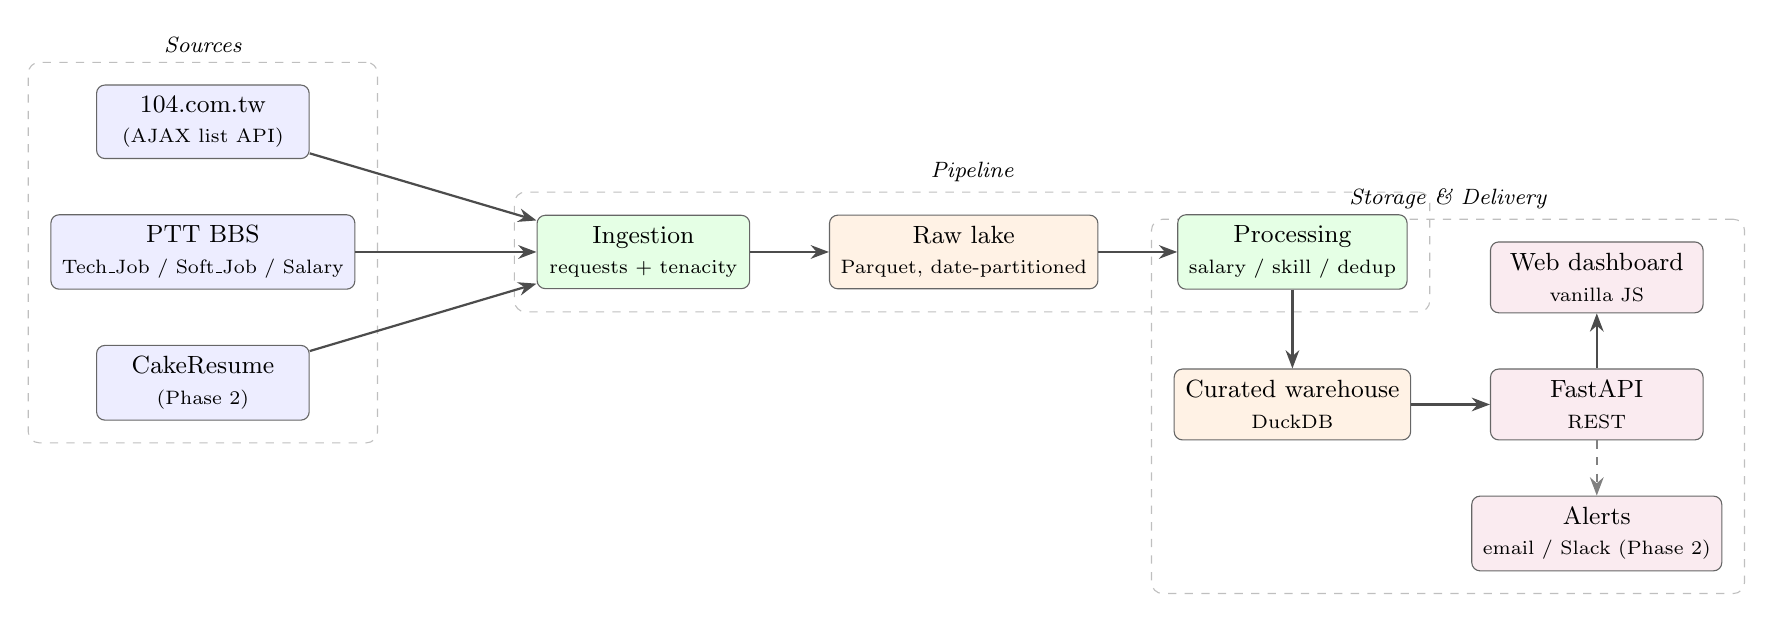
\begin{tikzpicture}[
  font=\small,
  node distance=0.7cm and 1.0cm,
  box/.style={
    rectangle, draw=black!60, rounded corners=3pt,
    minimum width=2.7cm, minimum height=0.9cm,
    align=center, inner sep=4pt,
  },
  source/.style={box, fill=blue!7},
  store/.style={box,  fill=orange!10},
  compute/.style={box,fill=green!10},
  serve/.style={box,  fill=purple!8},
  flow/.style={-Stealth, thick, draw=black!70},
  futureflow/.style={-Stealth, thick, draw=black!50, dashed},
  group/.style={rectangle, draw=black!25, dashed, rounded corners,
                inner sep=8pt, font=\footnotesize, fill=none},
]
\node[source]                       (s1) {104.com.tw\\\scriptsize (AJAX list API)};
\node[source, below=of s1]          (s2) {PTT BBS\\\scriptsize Tech\_Job / Soft\_Job / Salary};
\node[source, below=of s2]          (s3) {CakeResume\\\scriptsize (Phase 2)};

\node[compute, right=2.3cm of s2]   (ing) {Ingestion\\\scriptsize requests + tenacity};

\node[store, right=of ing]          (lake) {Raw lake\\\scriptsize Parquet, date-partitioned};

\node[compute, right=of lake]       (proc) {Processing\\\scriptsize salary / skill / dedup};

\node[store, below=of proc, yshift=-0.3cm] (wh) {Curated warehouse\\\scriptsize DuckDB};

\node[serve, right=of wh]           (api) {FastAPI\\\scriptsize REST};

\node[serve, above=of api]          (web) {Web dashboard\\\scriptsize vanilla JS};

\node[serve, below=of api]          (alert) {Alerts\\\scriptsize email / Slack (Phase 2)};

\draw[flow] (s1) -- (ing);
\draw[flow] (s2) -- (ing);
\draw[flow] (s3) -- (ing);
\draw[flow] (ing) -- (lake);
\draw[flow] (lake) -- (proc);
\draw[flow] (proc) -- (wh);
\draw[flow] (wh) -- (api);
\draw[flow] (api) -- (web);
\draw[futureflow] (api) -- (alert);

\begin{scope}[on background layer]
  \node[group, fit=(s1)(s2)(s3), label={[font=\footnotesize\itshape]above:Sources}] {};
  \node[group, fit=(ing)(lake)(proc), label={[font=\footnotesize\itshape]above:Pipeline}] {};
  \node[group, fit=(api)(web)(alert)(wh),
        label={[font=\footnotesize\itshape]above:Storage \& Delivery}] {};
\end{scope}
\end{tikzpicture}%
}
\caption{TalentScope TW pipeline. Solid edges are the implemented MVP;
dashed edges are the natural scale-out points discussed in
Section~\ref{sec:scalability}.}
\label{fig:arch}
\end{figure}

\subsection{Data sources}

\textbf{What actually works with pure HTTP (used in the MVP):}

\begin{itemize}[leftmargin=*,itemsep=0.1em,topsep=0.2em]
  \item \textbf{PTT} (\texttt{Tech\_Job}, \texttt{Soft\_Job},
    \texttt{Salary}) --- web scraping with BeautifulSoup over the
    public BBS HTML. We followed the 上頁 link to walk back ten
    index pages per board on 2026-06-16 and yielded 164 real
    salary-/offer-/請益-tagged posts whose body text we hydrated;
    those 164 records back Section~\ref{sec:evidence}.
\end{itemize}

\textbf{Documented but not used live --- a real GTM constraint:}

\begin{itemize}[leftmargin=*,itemsep=0.1em,topsep=0.2em]
  \item \textbf{104.com.tw.} The public AJAX endpoint
    (\texttt{/jobs/search/list}) is now behind Cloudflare's Bot
    Management challenge; plain \texttt{requests} returns 403, and
    \texttt{cloudscraper} silently degrades to the SPA shell HTML.
    Realistic production paths are (a) a Playwright/Chromium headless
    worker that solves the JS challenge before issuing the XHR, or
    (b) 104's paid B2B ``Job-Bank Data Service'' (NT\$50k--200k/yr).
    The MVP therefore uses a deterministic, plausibly-shaped
    synthetic dataset for end-to-end demo
    (\texttt{scripts/bootstrap\_sample\_data.py}); the parse code and
    schema in \texttt{src/ingestion/scrape\_104.py} are
    Playwright-migration-ready.
  \item \textbf{CakeResume / Yourator.} Both are Next.js SPAs whose
    job-listing endpoints render entirely client-side --- the
    ``\texttt{\_\_NEXT\_DATA\_\_}'' blob has the search shell but
    \texttt{pageMap} is empty until JS executes. Same Playwright
    constraint as 104.
\end{itemize}

The pivot here is itself a finding: a Taiwan SWE salary product has a
real ``picks-and-shovels'' moat opportunity, because the data
infrastructure (Playwright fleet + IP rotation + 104 API contract) is
exactly the kind of work an indie product cannot easily replicate.

\subsection{Ingestion}
\begin{itemize}[leftmargin=*,itemsep=0.1em,topsep=0.2em]
  \item Scrapers are plain \texttt{requests}-based for the MVP. The
    \texttt{PoliteClient} wrapper (\texttt{src/ingestion/http\_client.py})
    handles rate limiting, exponential-backoff retries via
    \texttt{tenacity}, and a recognisable User-Agent.
  \item Raw records land as date-partitioned Parquet under
    \texttt{data/raw/jobs} and \texttt{data/raw/ptt}; schema-on-read.
  \item At scale, this seam becomes a Kafka topic per source plus Spark
    Structured Streaming for late-arriving data --- the staging table
    never has to change.
\end{itemize}

\subsection{Storage}
\begin{itemize}[leftmargin=*,itemsep=0.1em,topsep=0.2em]
  \item \textbf{Raw lake.} Parquet (zstd) on local FS in the MVP; S3 / GCS
    with the same key layout in production.
  \item \textbf{Curated warehouse.} DuckDB. Tables: \texttt{raw\_jobs},
    \texttt{jobs}, \texttt{ptt\_salary\_mentions},
    \texttt{skills\_taxonomy}, \texttt{ingestion\_runs}. Indexes on
    \texttt{(role\_family, min\_yoe)},
    \texttt{(company\_normalized)}, \texttt{(posted\_at)}.
  \item \textbf{Why DuckDB at this scale?} The curated warehouse fits in
    well under a gigabyte. DuckDB gives us \texttt{quantile\_cont}, array
    operators (\texttt{list\_contains} for \texttt{skills}) and SQL
    portability for free; at 100$\times$ scale we would swap it for
    ClickHouse or BigQuery without touching the analytics SQL.
\end{itemize}

\subsection{Processing}
\begin{itemize}[leftmargin=*,itemsep=0.1em,topsep=0.2em]
  \item \textbf{Salary parser} (\texttt{src/processing/salary\_parser.py}).
    Handles 月薪 / 年薪, K-notation, 萬-notation, English ``Monthly NT\$X
    -- NT\$Y'' and the period-inference fallback for unannotated ranges.
    Confidence in $[0, 1]$. Coverage on the 8{,}000-record sample: \textbf{93.4\%}.
  \item \textbf{Skill extractor.} Curated taxonomy of 40 skills with
    aliases (e.g.\ \texttt{k8s}$\to$\texttt{kubernetes},
    \texttt{ts}$\to$\texttt{typescript}). Token-boundary aware to avoid
    \texttt{java} inside \texttt{javascript}.
  \item \textbf{Normalisation.} Title-rule regex $\to$ canonical role
    + family; company alias table (台積電 $\to$ TSMC); city extraction.
  \item \textbf{Deduplication.} SHA-1 fingerprint on
    (title, company, city).
  \item \textbf{Aggregations.} DuckDB \texttt{quantile\_cont} produces
    p10 / 25 / 50 / 75 / 90 per role, per skill, per company in $<5$\,ms
    on the sample.
  \item Batch-only for MVP; Flink or Kafka Streams when we add sub-minute
    alerts.
\end{itemize}

\subsection{Delivery}
\begin{itemize}[leftmargin=*,itemsep=0.1em,topsep=0.2em]
  \item \textbf{REST API} (FastAPI) at \texttt{/api/*}:
    \texttt{/benchmark}, \texttt{/skills/trending},
    \texttt{/companies/\{name\}}, \texttt{/me/underpaid},
    \texttt{/roles}, \texttt{/health}.
  \item \textbf{Web dashboard.} Vanilla-JS SPA mounted at \texttt{/}.
    Three widgets: salary benchmark form, ``am I underpaid?'' calculator,
    trending-skills table. Mobile-friendly.
  \item \textbf{Roadmap.} Email alerts for new postings that beat a saved
    benchmark; signed JSON exports for recruiter team subscriptions.
\end{itemize}

\subsection{Scalability \& cost}
\label{sec:scalability}

\begin{center}\small
\begin{tabular}{lrrll}
\toprule
\textbf{Scale} & \textbf{Active records} & \textbf{Cumulative} & \textbf{Stack} & \textbf{$\sim$Monthly cost} \\
\midrule
MVP (today)  &      8{,}000 & 8k     & 1 Fly.io VM + DuckDB           & US\$0   \\
10$\times$   &     80{,}000 & 200k   & + 1 worker, daily Spark batch  & US\$20  \\
100$\times$  &    800{,}000 & 5\,M   & Kafka, ClickHouse, 2 workers   & US\$200--400 \\
\bottomrule
\end{tabular}
\end{center}

Compute is cheap; \textbf{data acquisition is the cost driver}. A
Playwright-based scraping fleet (4 workers + residential proxies + headless
Chromium) is realistically US\$1{,}000--2{,}500/mo at the 10$\times$
scale, dwarfing the compute line. The unit-economics table below
(Section~\ref{sec:gtm}) reflects this.

\section{Go-to-market difficulties (Bonus)}
\label{sec:gtm}

\subsection*{Trust and adoption}
Engineers are skeptical by trade. ``How big is your sample?'' is the first
question; ``how do I know your parser is not broken?'' is the second.
\textbf{Mitigations:} every benchmark response carries its own
\texttt{sample\_size}; the API refuses to return percentiles under
$N{=}5$; the parser is open source so anyone can audit the regexes that
produced their number.

\subsection*{Data acquisition risk}
\emph{This was the biggest surprise of building the MVP.} The 2026-Q2
state of the Taiwan job-board ecosystem is that essentially every modern
listing site --- 104, CakeResume, Yourator, MeetJobs --- now requires a
real headless browser to retrieve any listing data. 104 is behind
Cloudflare Bot Management; CakeResume and Yourator are JS-rendered
SPAs whose initial HTML carries no job content. Pure HTTP scraping is
only viable on PTT.

This pushes data-acquisition cost from ``trivial cron + \texttt{requests}''
into the realm of Playwright fleets, IP rotation budgets, and CAPTCHA
solvers --- roughly NT\$30k--80k/month of operational cost at our target
Y1 scale. The realistic alternatives:

\begin{itemize}[leftmargin=*,itemsep=0.1em,topsep=0.2em]
  \item Paid B2B contract with 104's Data Service
    (NT\$50k--200k/yr) --- highest reliability, but you become
    economically dependent on a single source.
  \item Playwright-based scraping fleet on a residential proxy
    network --- $\sim$NT\$30k/mo at our scale, fragile, requires
    monthly maintenance as targets change selectors.
  \item Direct partnerships with smaller boards (CakeResume,
    MeetJobs, Yourator) --- might be willing to give us a data feed
    in exchange for traffic referral.
\end{itemize}

Counter-intuitively, the difficulty of the data side is itself a moat.
Any new entrant has the same scraping wall; only an incumbent with
contracts and infrastructure can run the product profitably at scale.

PTT is public and the over18 cookie is not a legal barrier; the bigger
challenge is extraction quality on a slang-heavy BBS. A small LLM
(Llama-3.1-8B) on the PTT body text would 2--3$\times$ our usable PTT
coverage, and is the obvious next investment.

\subsection*{Legal and privacy}
\begin{itemize}[leftmargin=*,itemsep=0.1em,topsep=0.2em]
  \item Personal Data Protection Act (PDPA) is satisfied because we never
    collect personal data: every demand-evidence source is a public
    posting; we run no surveys and do not solicit identifiable WTP.
  \item PTT post URLs are stored to make the pay-mention extractor
    auditable, but the author handle is not persisted into the
    curated warehouse.
  \item Individual salary numbers are never shown --- only percentile
    aggregates with $N\geq 5$.
  \item Posting copy is \copyright\ the employer; we store normalised
    structured fields (title, company, salary range, skills, city) but
    not the raw description in production.
\end{itemize}

\subsection*{Cold-start problem}
Unlike user-submitted-comp products (Levels.fyi, salary.tw), our supply
side is public scraping, so we are not chicken-and-egg. The critical mass
we need is $\approx$20k active postings --- enough to deliver $N\geq 10$
for the top 20 (role $\times$ city $\times$ yoe) buckets. 104 alone gets
us there in two weeks.

\subsection*{Competition and moats}
\begin{itemize}[leftmargin=*,itemsep=0.1em,topsep=0.2em]
  \item \textbf{104} has the data but is a job board, not a salary
    product; cultural inertia is real.
  \item \textbf{Levels.fyi} would need to invest in TW-specific scraping
    and a TW marketing presence. Possible, but slow.
  \item \textbf{Glassdoor} has been in maintenance mode for years.
  \item \textbf{Our moat} is product wedge + speed. The data is
    commodity; correctly framing ``am I underpaid'' for a specific
    Taiwan negotiation is not.
\end{itemize}

\subsection*{Unit economics}
\begin{itemize}[leftmargin=*,itemsep=0.1em,topsep=0.2em]
  \item Variable serving cost per query: $<$NT\$0.01.
  \item Fixed compute at MVP: $\sim$NT\$1,500/mo (Fly.io 1$\times$ VM
    + 1\,GB volume).
  \item Fixed data acquisition (the real cost): $\sim$NT\$30k--80k/mo
    once we move past PTT-only to include a Playwright fleet against
    104 / CakeResume / Yourator --- see Section~3 above.
  \item Break-even on PTT-only is $\sim$50 paid users at NT\$199/mo;
    break-even on the full data pipeline is closer to $\sim$300--500
    paid users. That is why Phase~1 of the GTM plan is PTT-only ---
    the unit economics are far friendlier before we incur scraping
    infrastructure cost.
  \item At 500 paid users with full pipeline: $\sim$NT\$20k--70k/mo
    gross margin; we are profitable but not yet hiring.
\end{itemize}

\section{Deployment (Bonus)}

The repository ships with three deploy paths:

\begin{itemize}[leftmargin=*,itemsep=0.1em,topsep=0.2em]
  \item \textbf{Fly.io} (preferred, Tokyo region): \texttt{fly launch
    --copy-config --name talentscope-tw} then \texttt{fly volumes create
    ts\_data --size 1} and \texttt{fly deploy}. The supplied
    \texttt{fly.toml} pins the smallest VM and auto-stops between
    requests, so monthly cost is US\$0--5 at MVP traffic.
  \item \textbf{Render}: push to GitHub, then ``New $+$ $\to$ Blueprint''
    on \texttt{render.yaml}; Render detects the Dockerfile and provisions
    the free tier.
  \item \textbf{Local Docker}: \texttt{docker compose up --build}.
\end{itemize}

\section{Reflection and what I would do next}

\begin{itemize}[leftmargin=*,itemsep=0.1em,topsep=0.2em]
  \item Replace the regex salary parser with a Llama-3.1-8B prompt; it
    would handle the long tail of free-text salary descriptions and push
    parser coverage above 98\%.
  \item Add a ``skill premium'' regression that controls for role, YoE
    and company tier --- a clean and defensible ML application.
  \item Run a real $\sim$50-user paid trial sourced via the same PTT
    channels we already scrape: post in \texttt{Tech\_Job} and
    \texttt{Soft\_Job}, offer a free baseline report in exchange for
    feedback, convert the high-intent subset to paid. No survey
    required.
  \item Add a Kafka topic + Spark Structured Streaming consumer once the
    data volume exceeds what a daily DuckDB batch handles comfortably
    (we project that is around 50k active postings).
\end{itemize}

The whole product is ``help me know what I am worth so I can negotiate
from a real number''. The technical system is deliberately boring ---
Parquet, DuckDB, FastAPI, vanilla JS --- because at this product stage
leverage comes from being correct and fast, not from being clever.

\vspace{1em}
\hrule\vspace{0.5em}
\small
\textbf{Repository:}\ \url{https://github.com/r14922020/talentscope-tw}
\quad \textbf{Demo:}\ \url{https://talentscope-tw.fly.dev}

\end{document}
